\documentclass{beamer}

\mode<presentation> {

%\usetheme{default}
%\usetheme{AnnArbor}
%\usetheme{Antibes}
%\usetheme{Bergen}
%\usetheme{Berkeley}
%\usetheme{Berlin}
%\usetheme{Boadilla}
%\usetheme{CambridgeUS}
%\usetheme{Copenhagen}
%\usetheme{Darmstadt}
%\usetheme{Dresden}
%\usetheme{Frankfurt}
%\usetheme{Goettingen}
%\usetheme{Hannover}
%\usetheme{Ilmenau}
%\usetheme{JuanLesPins}
%\usetheme{Luebeck}
\usetheme{Madrid}
%\usetheme{Malmoe}
%\usetheme{Marburg}
%\usetheme{Montpellier}
%\usetheme{PaloAlto}
%\usetheme{Pittsburgh}
%\usetheme{Rochester}
%\usetheme{Singapore}
%\usetheme{Szeged}
%\usetheme{Warsaw}


%\usecolortheme{albatross}
%\usecolortheme{beaver}
%\usecolortheme{beetle}
%\usecolortheme{crane}
%\usecolortheme{dolphin}
%\usecolortheme{dove}
%\usecolortheme{fly}
%\usecolortheme{lily}
%\usecolortheme{orchid}
%\usecolortheme{rose}
%\usecolortheme{seagull}
%\usecolortheme{seahorse}
%\usecolortheme{whale}
%\usecolortheme{wolverine}

%\setbeamertemplate{footline} % To remove the footer line in all slides uncomment this line
%\setbeamertemplate{footline}[page number] % To replace the footer line in all slides with a simple slide count uncomment this line

%\setbeamertemplate{navigation symbols}{} % To remove the navigation symbols from the bottom of all slides uncomment this line
}

\usepackage{graphicx} % Allows including images
\usepackage{booktabs} % Allows the use of \toprule, \midrule and \bottomrule in tables
\usepackage{amsfonts}
\usepackage{mathrsfs}
\usepackage{amsmath,amssymb,graphicx}

\newcommand{\verbatimfont}[1]{\renewcommand{\verbatim@font}{\ttfamily#1}} % small verbatim

%----------------------------------------------------------------------------------------
%	TITLE PAGE
%----------------------------------------------------------------------------------------

\title["1.5"]{1.5: Estimation and Elimination of Trend and Seasonal Components} 

\author{Taylor} 
\institute[UVA] 
{
University of Virginia \\
\medskip
\textit{} 
}
\date{} 

\begin{document}
%----------------------------------------------------------------------------------------

\begin{frame}
\titlepage 
\end{frame}
%----------------------------------------------------------------------------------------

\begin{frame}
\frametitle{Motivation}

All the material from last chapter was only for {\bf stationary} time series only!
\newline

Before you use all of that:
\begin{enumerate}
\item plot the series (does it look stationary?)
\item Does it need to be broken up into homogeneous segments?
\item Do we need to discard outliers? Incorrectly recorded?
\item Do we need to decompose the data into trend, seasonal component and stationary component?
\item Do we need to transform the data? Take the logarithm? Take Differences? Take percents changes?
\end{enumerate}

\end{frame}




%----------------------------------------------------------------------------------------

\begin{frame}
\frametitle{Definition}

\begin{block}{Approach 1: Classical Decomposition Model}
The {\bf classical decomposition model} for a series $\{X_t\}$ is written as
\[
X_t = m_t + s_t + Y_t,
\]
where
\begin{enumerate}
\item $m_t$ is the slowly changing trend component
\item $s_t$ is the seasonal component with known frequency/period
\item $Y_t$ is weakly stationary noise (something from last chapter)
\end{enumerate}
\end{block}


%A competitor to the classical decomposition model is the {\bf differencing approach}. 


\end{frame}

%----------------------------------------------------------------------------------------

\begin{frame}
\frametitle{Nota Bene}

Transforming the data by taking the log of each $x_t$ is commonly done if the seasonal and noise
fluctuations appear to increase with the level of the process.

\begin{center}
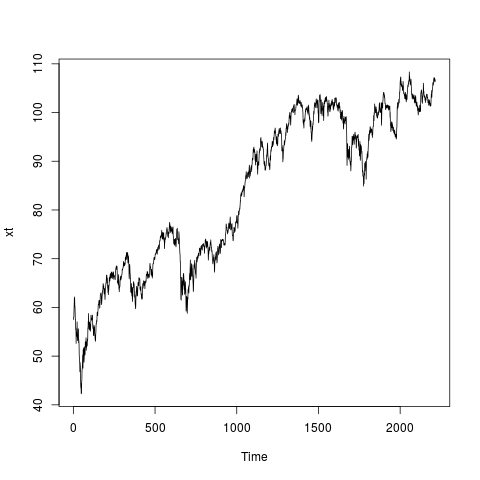
\includegraphics[width=60mm]{/home/taylor/UVa/all_teaching/4170_slides/1/1.5/pics/Rplot}
\end{center}


\end{frame}

%----------------------------------------------------------------------------------------

\begin{frame}
\frametitle{Definition}

With financial time series, people are usually interested in returns
\begin{itemize}
\item continuously compounded: $R_t = \log(X_t) - \log(X_{t-1})$
\item compounded weekly, daily, etc.: $S_t = \left( \frac{X_t - X_{t-1} }{X_{t-1}} \right) = X_t/X_{t-1} - 1$
\end{itemize}

Running ``Wealth":
\begin{itemize}
\item Taking the log of each time point is looking at the cumulative sum of the first one
\item You can take the arithmetic everage of the log returns $\sum_{t=1}^T R_t / T$
\item If you don't look at continuously compounded returns, you want the geometric average: $(\prod_{t=1}^T [1+S_t])^{1/T}$
\item We usually take the log 
\end{itemize}

\end{frame}

%----------------------------------------------------------------------------------------

\begin{frame}
\frametitle{Fitting the trend?}

If our model is 
\[
X_t = m_t + s_t + Y_t,
\]
how do we get an idea of $m_t$ and $s_t$?
\newline

First, let's assume $s_t = 0$.
\end{frame}

%----------------------------------------------------------------------------------------

\begin{frame}
\frametitle{Method 1: Smoothing with finite moving average filter}

Assume the model is 
\[
X_t = m_t + Y_t, \hspace{10mm} t=1,\ldots,n
\]
with $E[Y_t]=0$, then define
\[
W_t = \frac{1}{2q+1}\sum_{j=-q}^qX_{t-j}.
\]
Why? Because the mean shows up better and the noise is attenuated. 
\[
W_t = \frac{1}{2q+1}\sum_{j=-q}^q m_{t-j} + \frac{1}{2q+1}\sum_{j=-q}^q Y_{t-j} \approx \frac{1}{2q+1}\sum_{j=-q}^q m_{t-j}
\]
for $q + 1 \le t \le n - q$ because $\frac{1}{2q+1}\sum_{j=-q}^q Y_{t-j} \to 0$ by the law of large numbers.

\end{frame}

%----------------------------------------------------------------------------------------

\begin{frame}
\frametitle{Method 1: Smoothing with finite moving average filter}

\begin{center}
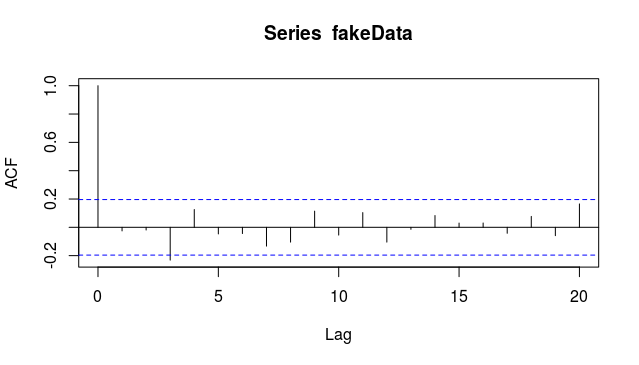
\includegraphics[width=100mm]{/home/taylor/UVa/all_teaching/4170_slides/1/1.5/pics/Rplot01}
\end{center}

Be careful though. Applying {\bf linear filters} might wash away the trend component too!

\end{frame}

%----------------------------------------------------------------------------------------

\begin{frame}
\frametitle{Method 2: Exponential Smoothing}

Assume the model is 
\[
X_t = m_t + Y_t, \hspace{10mm} t=1,\ldots,n
\]
with $E[Y_t]=0$ again. Then pick $\alpha \in [0,1]$. Finally define the mean estimate recursively:
\[
\hat{m}_t = \alpha X_t + (1-\alpha) \hat{m}_{t-1}
\]
with the initial condition $\hat{m}_1 = x_1$.
\newline

They call it exponential smoothing because the weights decrease exponentially:
\begin{align*}
\hat{m}_t &= \alpha X_t + (1-\alpha)[\alpha X_{t-1} + (1-\alpha)\hat{m}_{t-2}] \\
&= \alpha X_t + \alpha (1-\alpha) X_{t-1} + (1-\alpha)^2 [\alpha X_{t-2} + (1-\alpha)\hat{m}_{t-3}]\\
&= \alpha \sum_{j=0}^{t-2}(1-\alpha)^jX_{t-j} + (1-\alpha)^{t-1}X_1
\end{align*}

\end{frame}

%----------------------------------------------------------------------------------------

\begin{frame}
\frametitle{Method 2: Exponential Smoothing}

\begin{center}
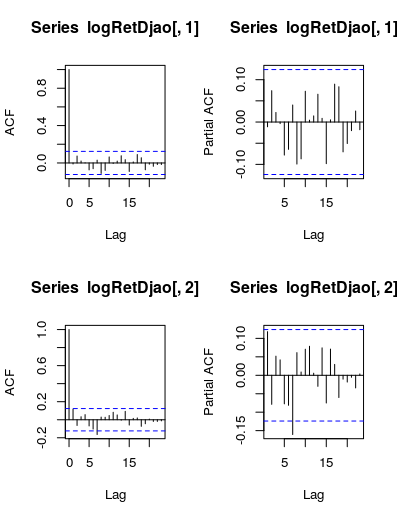
\includegraphics[width=110mm]{/home/taylor/UVa/all_teaching/4170_slides/1/1.5/pics/Rplot02}
\end{center}

\end{frame}

%----------------------------------------------------------------------------------------

\begin{frame}
\frametitle{Methods 3 \& 4}

We can also
\begin{enumerate}
\item Smooth by fitting a Fourier series that lacks high frequency components
\item Smooth by fitting a polynomial to the data
\end{enumerate}
More on these later...
\end{frame}

%----------------------------------------------------------------------------------------

\begin{frame}
\frametitle{Method 4}
\begin{center}
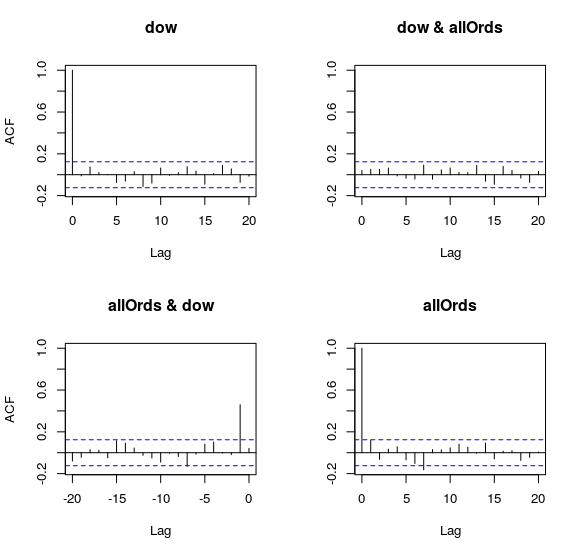
\includegraphics[width=90mm]{/home/taylor/UVa/all_teaching/4170_slides/1/1.5/pics/Rplot03}
\end{center}
Equivalent to assuming
\[
\log(P_t) = \beta_0 + \beta_1 t + W_t \text{  OR  } \log(P_t) - \log(P_{t-1}) = \beta_1 + W_t - W_{t-1}
\]
or that the log returns are IID $\text{Normal}(\beta_1, 2 \sigma^2)$.
\end{frame}

%----------------------------------------------------------------------------------------

\begin{frame}
\frametitle{Preliminary Definitions}

\begin{block}{The Backshift Operator}
The {\bf backshift operator}, denoted by $B$, means
\[
B X_t = X_{t-1}. 
\]
\end{block}
Note that $B^2 = BX_{t-1} = X_{t-2}$ and so on.

\begin{block}{The Differencing Operator}
The {\bf differencing operator}, denoted by $\nabla$, means
\[
\nabla X_t = X_t - X_{t-1} = (1-B)X_t
\]
\end{block}
Note that $\nabla^2 X_t = \nabla (1-B)X_t = (1 - 2B + B^2)X_t = X_t - 2 X_{t-1} + X_{t-2}$, and so on.

\end{frame}

%----------------------------------------------------------------------------------------

\begin{frame}
\frametitle{Approach 2: Trend Elimination by Differencing}


\begin{block}{Approach 2: Trend Elimination by Differencing}
The {\bf differencing method} attempts to detrend the data by differencing the time series, and fitting a stationary model on the differenced series $\nabla^k X_t$, for some $k$.
\end{block}
%A competitor to the classical decomposition model is the {\bf differencing approach}. 

Example: Assume $X_t = a_0 + a_1 t + a_2 t^2 + Y_t$. 
\begin{align*}
\nabla X_t &= a_1 + 2 a_2 t - a_2 + \nabla Y_t \\
\nabla^2 X_t &= 2 a_2 + \nabla^2 Y_t
\end{align*}
So we would model $\nabla^2 X_t$ with a stationary time series model from last chapter.
\end{frame}


%----------------------------------------------------------------------------------------

\begin{frame}
\frametitle{Differencing Example}

Differencing once gives us the log returns.

\begin{center}
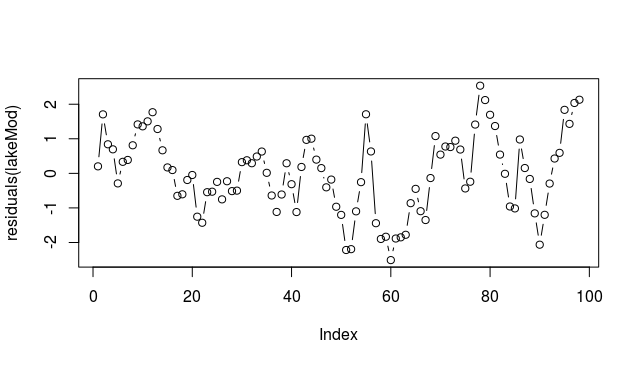
\includegraphics[width=100mm]{/home/taylor/UVa/all_teaching/4170_slides/1/1.5/pics/Rplot04}
\end{center}

\end{frame}

%----------------------------------------------------------------------------------------

\begin{frame}
\frametitle{Fitting the trend?}

If our model is 
\[
X_t = m_t + s_t + Y_t,
\]
how do we get an idea of $m_t$ and $s_t$?
\newline

Now, let's assume $s_t \neq 0$. Specifically, let $s_{t+d} = s_t$ and $\sum_{j=1}^d s_j = 0$, for some period $d$.
\end{frame}

%----------------------------------------------------------------------------------------

\begin{frame}
\frametitle{Method S1: Estimation of Trend and Seasonal Components}

If our model is 
\[
X_t = m_t + s_t + Y_t,
\]

Step 1: Estimate $m_t$ with $\hat{m}_t$. $d$ is the period. 
\begin{itemize}
\item If $d=2q$, then $\hat{m}_t = (.5 x_{t-q} + x_{t-q+1} + \cdots + x_{t+q-1} + .5 x_{t+q})/d$
\item If $d=2q+1$, then $\hat{m}_t = (\sum_{i=-q}^q x_{t-i})/(2q+1)$
\end{itemize}
for $q < t \le n-q$
\end{frame}

%----------------------------------------------------------------------------------------

\begin{frame}
\frametitle{Method S1: Estimation of Trend and Seasonal Components}

If our model is 
\[
X_t = m_t + s_t + Y_t,
\]

Step 2: Estimate $s_t$ with $\hat{s}_t$. For times $k=1,\ldots,d$
\begin{itemize}
\item $w_k = \text{mean}_{j}( x_{k+jd} - \hat{m}_{k+jd} ) $
\item $\hat{s}_k = w_k - d^{-1}\sum_{i=1}^d w_i$ 
\item $\hat{s}_l = \hat{s}_{l-d}$ for $l > d$
\end{itemize}
for $q < k + jd \le n-q$

\end{frame}

%----------------------------------------------------------------------------------------

\begin{frame}
\frametitle{Method S1: Estimation of Trend and Seasonal Components}

If our model is 
\[
X_t = m_t + s_t + Y_t,
\]

Step 3: Deseasonalize the data
\begin{itemize}
\item $d_t = x_t - \hat{s}_t$
\end{itemize}
for $0 < t \le n$
\newline

Step 4: Re-estimate the trend $m_t$
\begin{itemize}
\item Use a method that we talked about in the prior section on the series $d_t$
\end{itemize}
\end{frame}

%----------------------------------------------------------------------------------------

\begin{frame}[fragile]
\frametitle{Method S2: Elimination of Trend and Seasonal Components
by Differencing}

If our model is 
\[
X_t = m_t + s_t + Y_t,
\]
then
\[
\nabla_d X_t = m_t - m_{t-d} + Y_t - Y_{t-d}
\]
where $\nabla_d$ is the lag-d difference, (not $\nabla^d$!)
\newline

In R:
\begin{verbatim}
diff(logRets, lag=12)
\end{verbatim}

Note that $\nabla \nabla_d X_t = \nabla_d \nabla X_t$, but it's recommended that you apply $\nabla_d$ first (left side).

\end{frame}





\end{document} 